\documentclass[11pt,a4paper,oneside]{article} % dock basic params

% Ru lang stuff
    \usepackage [utf8x] {inputenc}
    \usepackage [T2A] {fontenc}

% running titles 
    \usepackage{fancybox}
    \usepackage{fancyhdr}
    
% for last page number
    \usepackage{lastpage}

%for colored tablets cells
    \usepackage{colortbl}

% for Ru text in formulas
    \usepackage[warn]{mathtext}

% for captions 
    \usepackage[labelsep=period]{caption}

% for colored hyperrefs
    \usepackage{xcolor}
    \usepackage{hyperref}
    
% for pictures 
    \usepackage{graphicx}

% for coll math
    \usepackage{amsmath}

% path to all pictures
    \graphicspath{{picks/}}

% for enumerates
    \usepackage[shortlabels]{enumitem}

% for diff running titles on pages with diff parity
    \usepackage{ifthen}
    \usepackage{pdfpages}
    \usepackage[strict]{changepage}

%for drawings
    \usepackage{tikz}
    \usetikzlibrary{calc}
    \usetikzlibrary{decorations.pathmorphing}

% for good text in tablets
    \usepackage{array}
    \newcolumntype{P}[1]{>{\centering\arraybackslash}p{#1}}
    
% dock fields 20 15 15 35
    \usepackage[left=12mm, top=12mm, right=15mm, bottom=28mm, nohead, footskip=10mm]{geometry}
    
% for cool tables
    \usepackage{multirow}


% for different section/subsection/subsubsection styles in contents and doc

        \newcommand{\sect}[2] {
            \addtocounter{section}{1}
            \section*{\Huge\thesection.\,#1}
            \addcontentsline{toc}{subsection}{ \texorpdfstring{\thesection.\qquad\qquad #2}{Lg}}
        }
        
        \newcommand{\subsec}[2] {
            \addtocounter{subsection}{1}
            \subsection*{\thesubsection.\,#1}
            \addcontentsline{toc}{subsection}{ \texorpdfstring{\quad \thesubsection.\qquad\ #2}{Lg}}
        }
        
        \newcommand{\subsubsec}[2] {
            \addtocounter{subsubsection}{1}
            \subsubsection*{\thesubsubsection.\,#1}
            \addcontentsline{toc}{subsection}{ \texorpdfstring{\quad\quad\ \thesubsubsection. #2}{Lg}}
        }
%-------------------------------------------------------------------------%


% for easy mini pages with shifts
    \newcommand{\shiftedText}[3]{
    \hspace*{#1}\begin{minipage}[t]{#2}
        #3
    \end{minipage}
    }

% for lab number change in all doc
    \newcommand{\labnum}{
        6.1
    }

% page style setup (for running titles)
    \fancypagestyle{plain}{ %
    	\fancyhf{} % remove everything
    	
    	 % lines parameters
    	\renewcommand{\headrulewidth}{0pt}
    	\renewcommand{\footrulewidth}{0pt}
    	
    	% running titles contents
    	\fancyfoot[L]{\ifthenelse{\isodd{\thepage}}{Работа \labnum}{\thepage}}
    	\fancyfoot[R]{\ifthenelse{\isodd{\thepage}}{\thepage}{Работа \labnum}}
    }

% choosing page style with our running titles
    \pagestyle{plain}

\tolerance = 10000

% DOC BODY
\begin{document}
     % table of contents numeral depth
	    \setcounter{tocdepth}{4}
	
	% all counters setup
    	\setcounter{section}{0}
    	\setcounter{subsection}{0}
    	\setcounter{subsubsection}{0}
    	
    % some text placement parameters
    	\textheight = 240mm
    	\footskip = 10mm
        \leftskip = 10mm
    
    % add title page
    	
%!!! Just custom title stuff here !!!%

\shiftedText{0.5cm}{14cm}
{

    \begin{center}
    \vspace*{1.0cm}    
        
        {\bf\huge Работа \labnum }
        
    \vspace*{0.4cm}    
        
        {\bf\Large РАСПРЕДЕЛЕНИЕ ДАННЫХ В ХЭШ ТАБЛИЦЕ }
        
    \vspace*{0.8cm}
        
        {\Large Работу выполнил Матренин Василий Б01-006 }
        
    \vspace*{1.6cm}
    \end{center}
    
    {\bf\noindent Цель работы: }Реализовать свою хэш таблицу и протестировать распределение элементов из тестовой выборки по спискам хэш таблицы
    
    \vspace*{0.6cm}
    
    {\bf\noindent В работе использовались: }Ноутбук, мозг, пол пачки мятных пряников, 2 стакана кофе 
    
}

\newpage
    	
    % fixing running titles shifts after title page
    	\headheight = 0.5cm
    	\headsep = 1.2cm
    
	% other file input
    	
\section{ Распределения }
На рисунках 1-6 представлены графики для различных хэш функций:

\noindent\begin{minipage}[h!]{0.45\linewidth}
    \begin{center}
        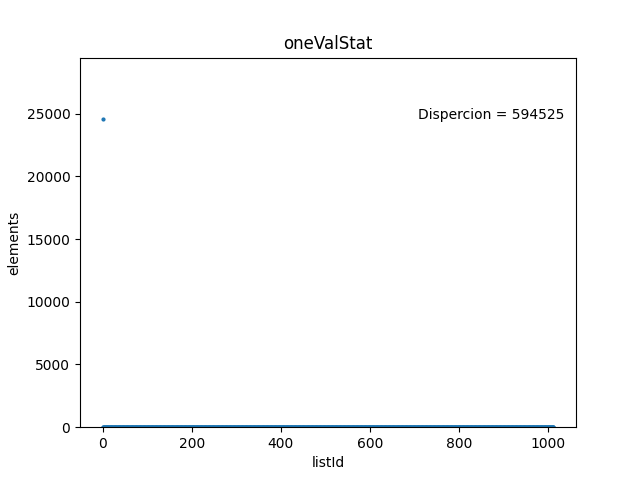
\includegraphics[width = 1\linewidth]{oneValStat.png} \\
        \textit{Рис. 1. хэш функция одного значения }
    \end{center} 
\end{minipage}
\begin{minipage}[h!]{0.45\linewidth}
    \begin{center}
        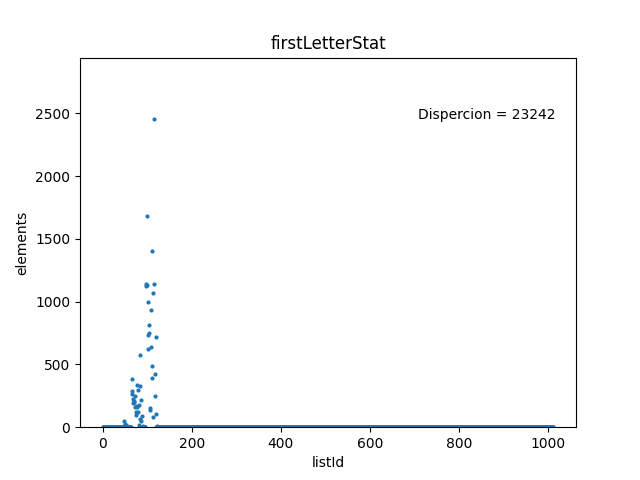
\includegraphics[width = 1\linewidth]{firstLetterStat.png} \\
        \textit{Рис. 2. хэш функция первой буквы }
    \end{center} 
\end{minipage}

\noindent\begin{minipage}[h!]{0.45\linewidth}
    \begin{center}
        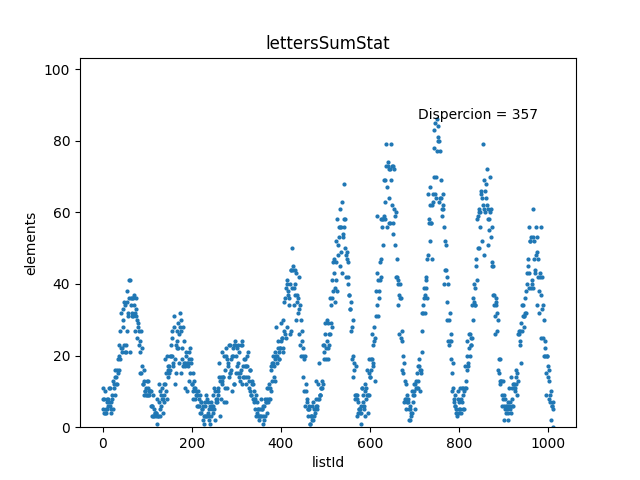
\includegraphics[width = 1\linewidth]{lettersSumStat.png} \\
        \textit{Рис. 3. хэш функция суммы букв }
    \end{center} 
\end{minipage}
\begin{minipage}[h!]{0.45\linewidth}
    \begin{center}
        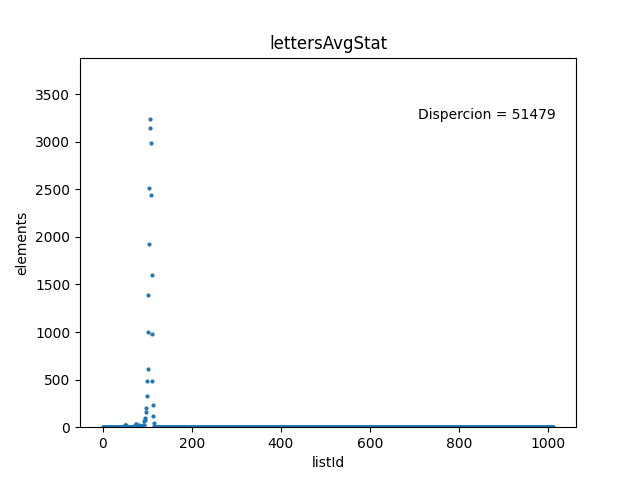
\includegraphics[width = 1\linewidth]{lettersAvgStat.png} \\
        \textit{Рис. 4. хэш функция среднего значения\\ кодов символов }
    \end{center} 
\end{minipage}

\noindent\begin{minipage}[h!]{0.45\linewidth}
    \begin{center}
        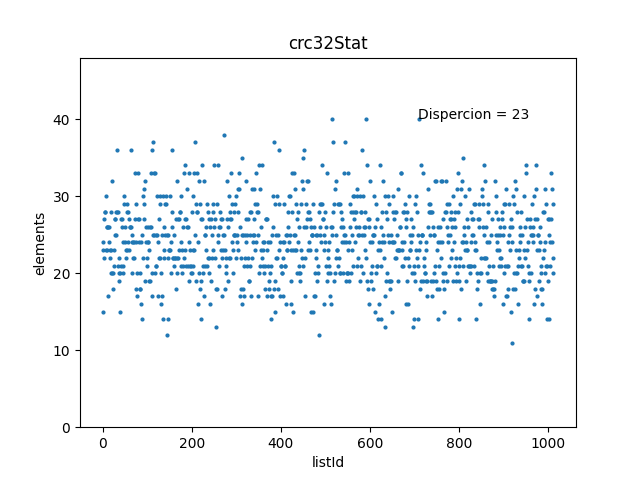
\includegraphics[width = 1\linewidth]{crc32Stat.png} \\
        \textit{Рис. 5. crc32 }
    \end{center} 
\end{minipage}
\noindent\begin{minipage}[h!]{0.45\linewidth}
    \begin{center}
        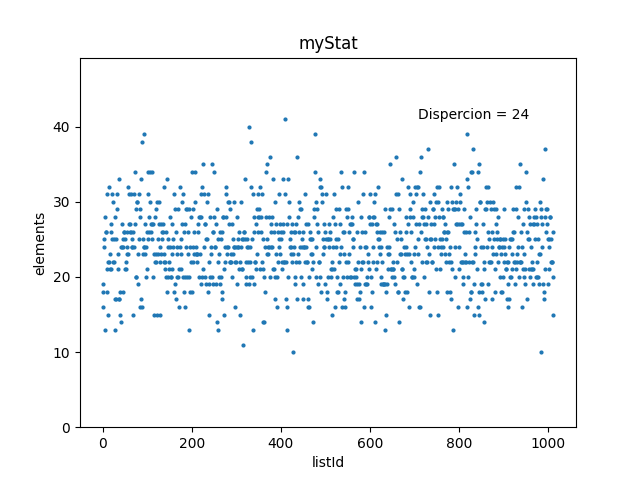
\includegraphics[width = 1\linewidth]{myStat.png} \\
        \textit{Рис. 6. моя хэш функция из 1 семестра }
    \end{center} 
\end{minipage}

\newpage

\section{ Вывод }

Хочется отметить, что моя хэш функция из 1 семестра работает на равне с crc32 (по распределению). \\ [0.1cm]
Видно, что лучше всего себя показывает crc32. Его я и буду использовать для следующей лабараторной работы.

\end{document}